\section{infofieldenter Class Reference}
\label{classinfofieldenter}\index{infofieldenter@{infofieldenter}}
{\tt \#include $<$infofieldenter.h$>$}

\subsection*{Public Slots}
\begin{CompactItemize}
\item 
void {\bf expand\_\-info\_\-click} (void)
\end{CompactItemize}
\subsection*{Public Member Functions}
\begin{CompactItemize}
\item 
{\bf infofieldenter} (QWidget $\ast$parent=0)
\item 
{\bf $\sim$infofieldenter} ()
\item 
void {\bf set\_\-focus\_\-to\_\-start} (void)
\item 
bool {\bf check\_\-field\_\-name} (QString name)
\item 
QString {\bf get\_\-field} (QString name)
\item 
void {\bf set\_\-field} (QString name, QString value)
\end{CompactItemize}
\subsection*{Private Member Functions}
\begin{CompactItemize}
\item 
void {\bf setup\_\-ui} (void)
\item 
void {\bf setup\_\-signals} (void)
\item 
void {\bf assembly} (void)
\item 
void {\bf expand\_\-info\_\-on\_\-display} (QString expand)
\end{CompactItemize}
\subsection*{Private Attributes}
\begin{CompactItemize}
\item 
QLabel $\ast$ {\bf recordname\_\-label}
\item 
QLine\-Edit $\ast$ {\bf recordname}
\item 
QLabel $\ast$ {\bf recordauthor\_\-label}
\item 
QLine\-Edit $\ast$ {\bf recordauthor}
\item 
QLabel $\ast$ {\bf recordurl\_\-label}
\item 
QLine\-Edit $\ast$ {\bf recordurl}
\item 
QLabel $\ast$ {\bf recordtags\_\-label}
\item 
QLine\-Edit $\ast$ {\bf recordtags}
\item 
QTool\-Button $\ast$ {\bf expand\_\-info}
\item 
QGrid\-Layout $\ast$ {\bf infofieldlayout}
\end{CompactItemize}


\subsection{Detailed Description}




Definition at line 15 of file infofieldenter.h.

\subsection{Constructor \& Destructor Documentation}
\index{infofieldenter@{infofieldenter}!infofieldenter@{infofieldenter}}
\index{infofieldenter@{infofieldenter}!infofieldenter@{infofieldenter}}
\subsubsection{\setlength{\rightskip}{0pt plus 5cm}infofieldenter::infofieldenter (QWidget $\ast$ {\em parent} = {\tt 0})}\label{classinfofieldenter_4a1d31e749d90f7d36ea594e383e05bc}




Definition at line 10 of file infofieldenter.cpp.

References assembly(), setup\_\-signals(), and setup\_\-ui().

Here is the call graph for this function:\begin{figure}[H]
\begin{center}
\leavevmode
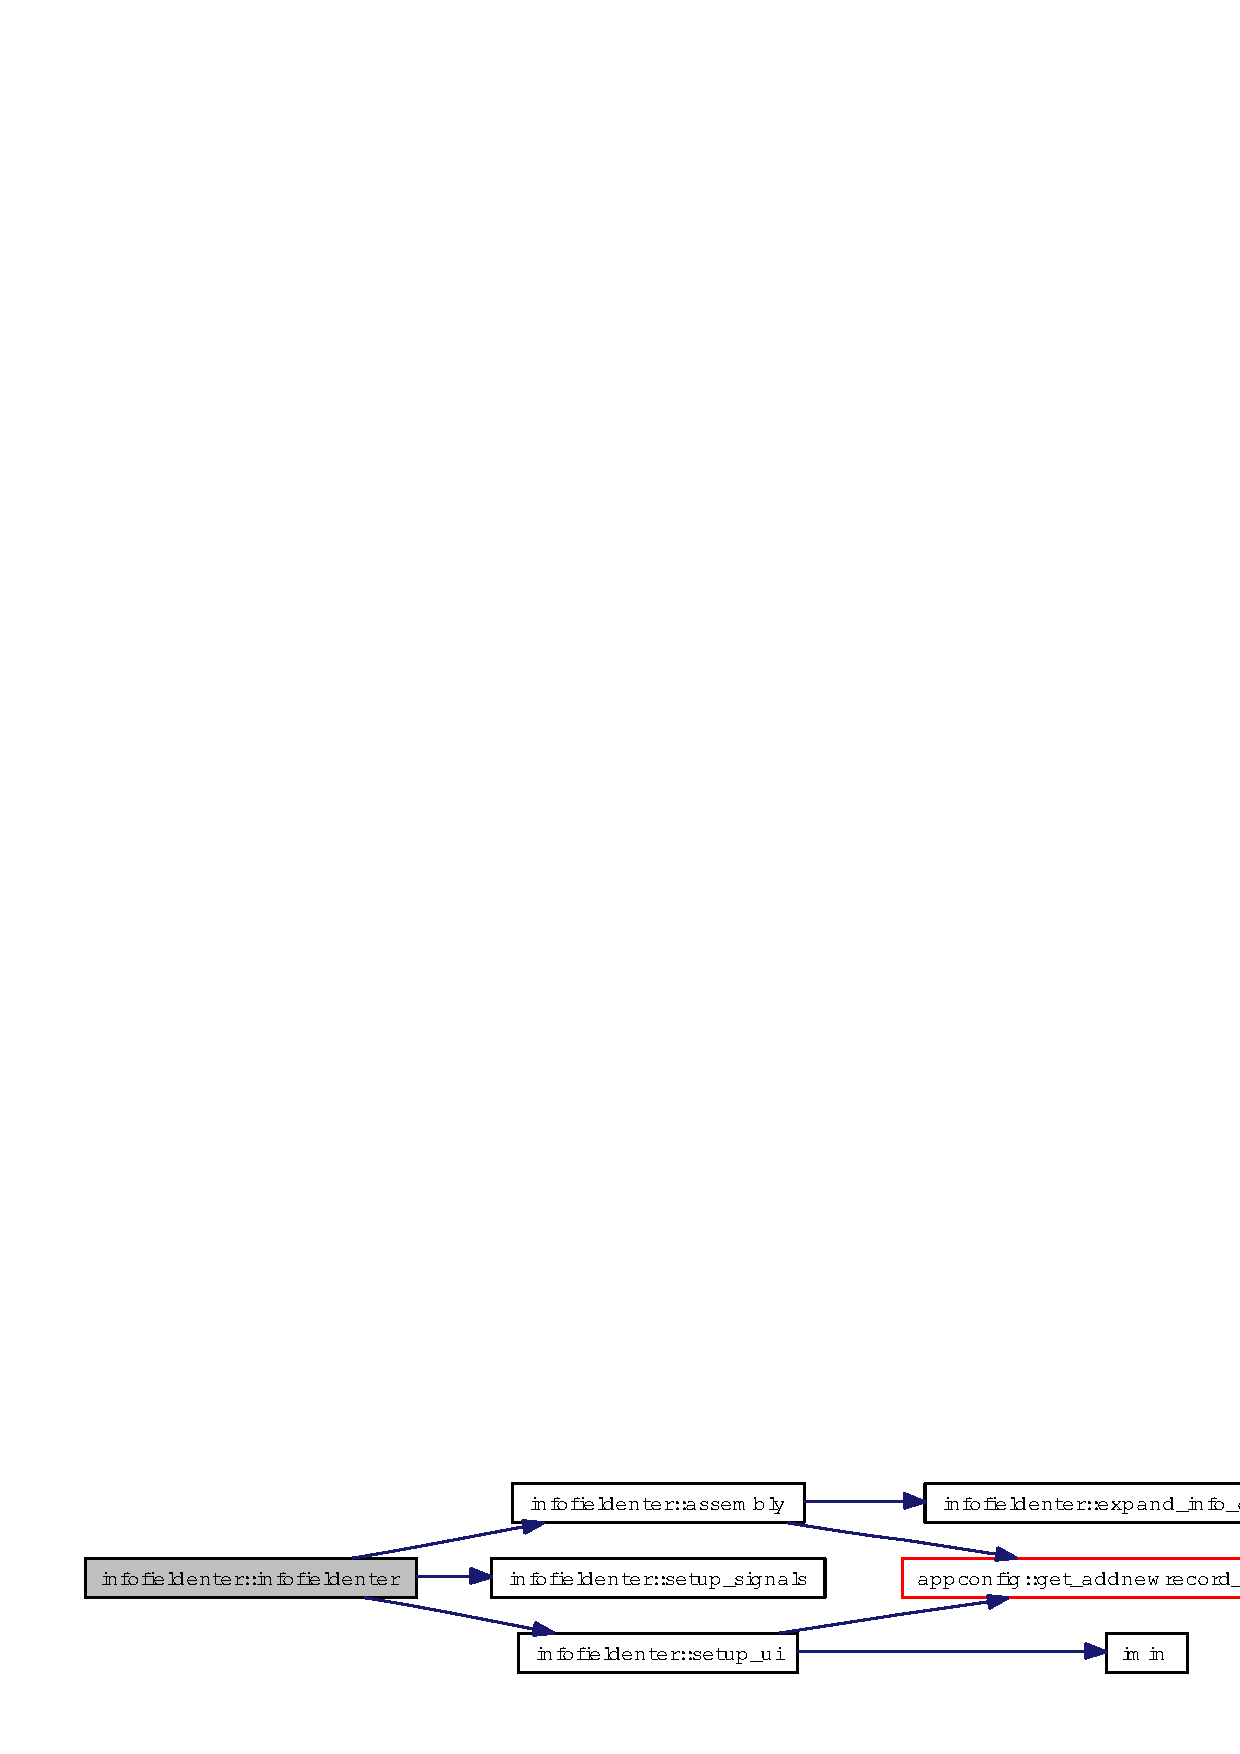
\includegraphics[width=336pt]{classinfofieldenter_4a1d31e749d90f7d36ea594e383e05bc_cgraph}
\end{center}
\end{figure}
\index{infofieldenter@{infofieldenter}!~infofieldenter@{$\sim$infofieldenter}}
\index{~infofieldenter@{$\sim$infofieldenter}!infofieldenter@{infofieldenter}}
\subsubsection{\setlength{\rightskip}{0pt plus 5cm}infofieldenter::$\sim$infofieldenter ()}\label{classinfofieldenter_dc661d7f68f42cd5e280e0cab8bb5890}




Definition at line 17 of file infofieldenter.cpp.

\subsection{Member Function Documentation}
\index{infofieldenter@{infofieldenter}!set_focus_to_start@{set\_\-focus\_\-to\_\-start}}
\index{set_focus_to_start@{set\_\-focus\_\-to\_\-start}!infofieldenter@{infofieldenter}}
\subsubsection{\setlength{\rightskip}{0pt plus 5cm}void infofieldenter::set\_\-focus\_\-to\_\-start (void)}\label{classinfofieldenter_29b36d24b6f15fb60140f4289025a4ee}




Definition at line 153 of file infofieldenter.cpp.

References recordname.

Referenced by editrecord::assembly(), and addnewrecord::assembly().

Here is the caller graph for this function:\begin{figure}[H]
\begin{center}
\leavevmode
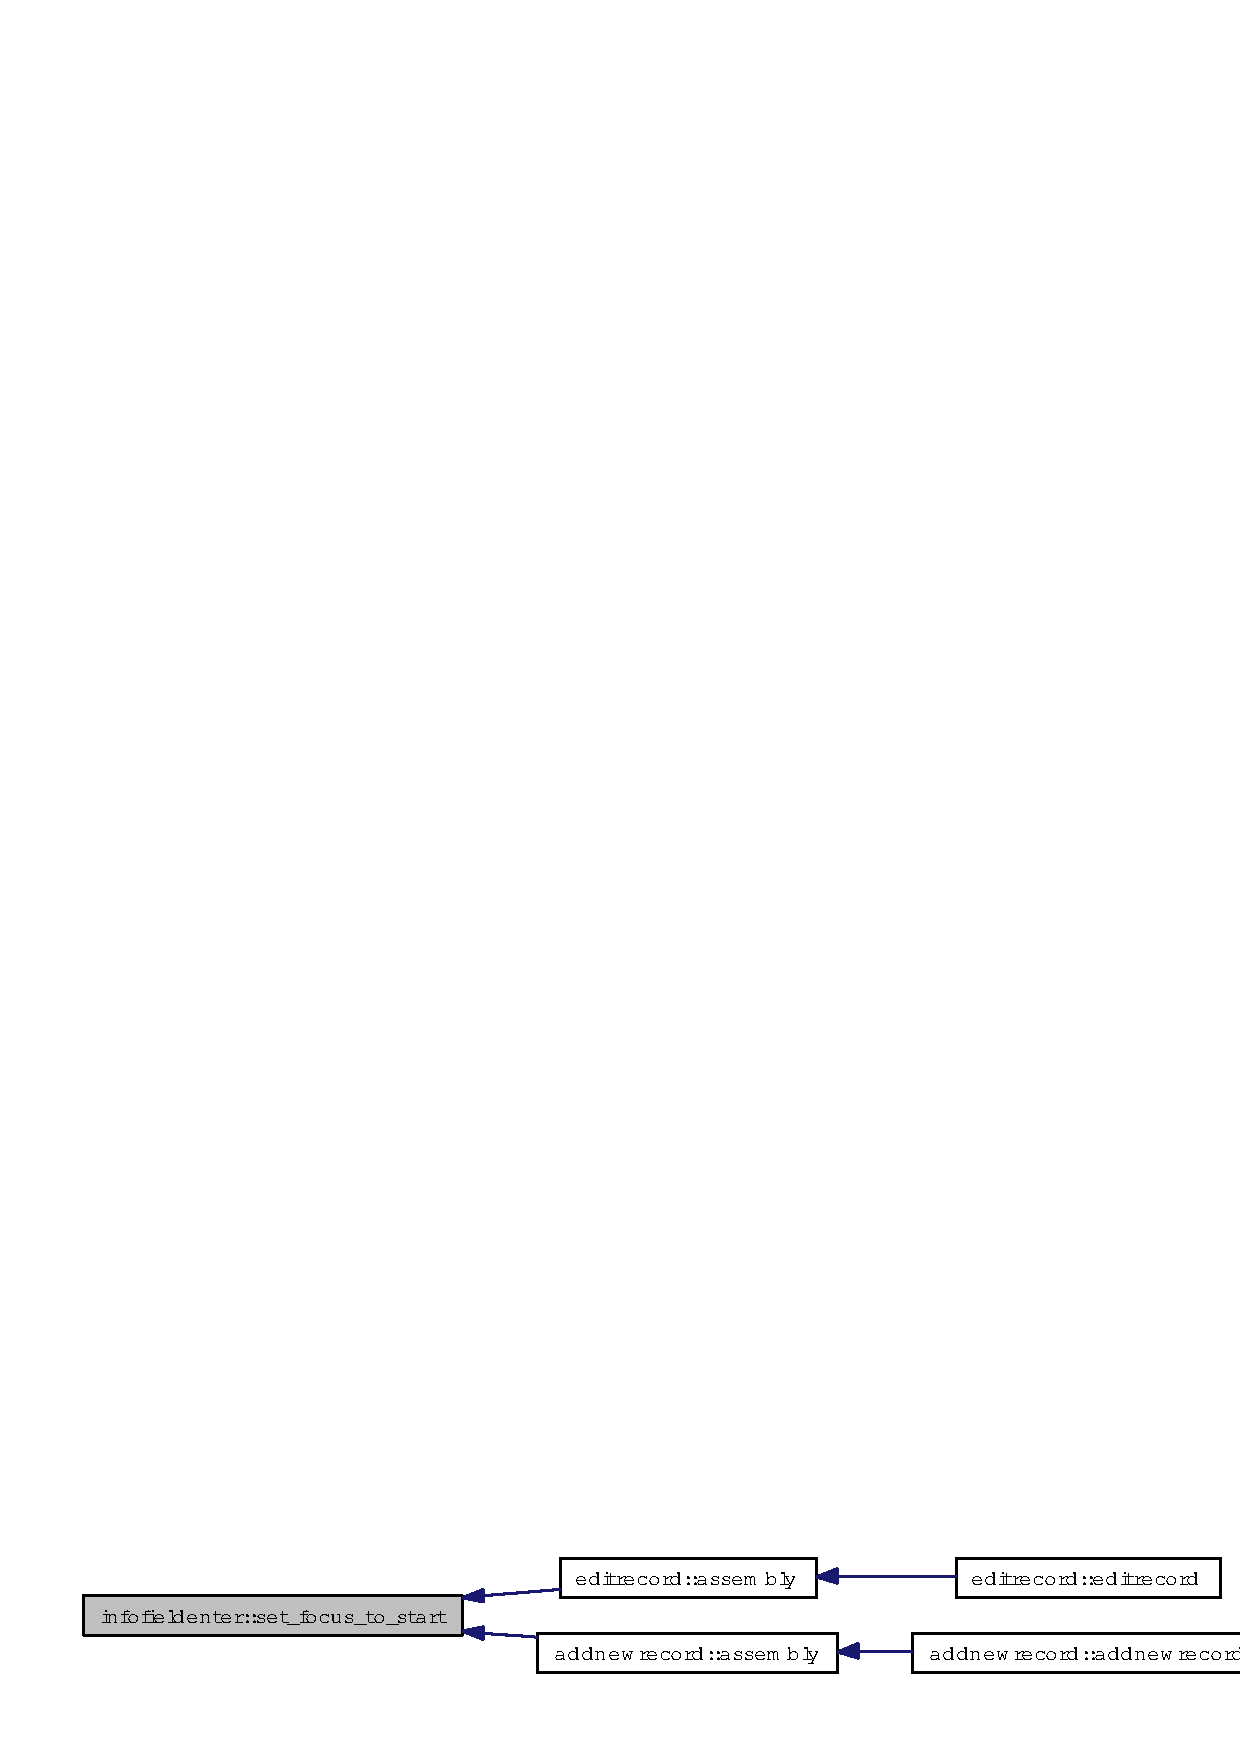
\includegraphics[width=305pt]{classinfofieldenter_29b36d24b6f15fb60140f4289025a4ee_icgraph}
\end{center}
\end{figure}
\index{infofieldenter@{infofieldenter}!check_field_name@{check\_\-field\_\-name}}
\index{check_field_name@{check\_\-field\_\-name}!infofieldenter@{infofieldenter}}
\subsubsection{\setlength{\rightskip}{0pt plus 5cm}bool infofieldenter::check\_\-field\_\-name (QString {\em name})}\label{classinfofieldenter_1020b1777a4f93a10b5c04308625e62c}




Definition at line 158 of file infofieldenter.cpp.

Referenced by get\_\-field(), editrecord::get\_\-field(), set\_\-field(), and editrecord::set\_\-field().

Here is the caller graph for this function:\begin{figure}[H]
\begin{center}
\leavevmode
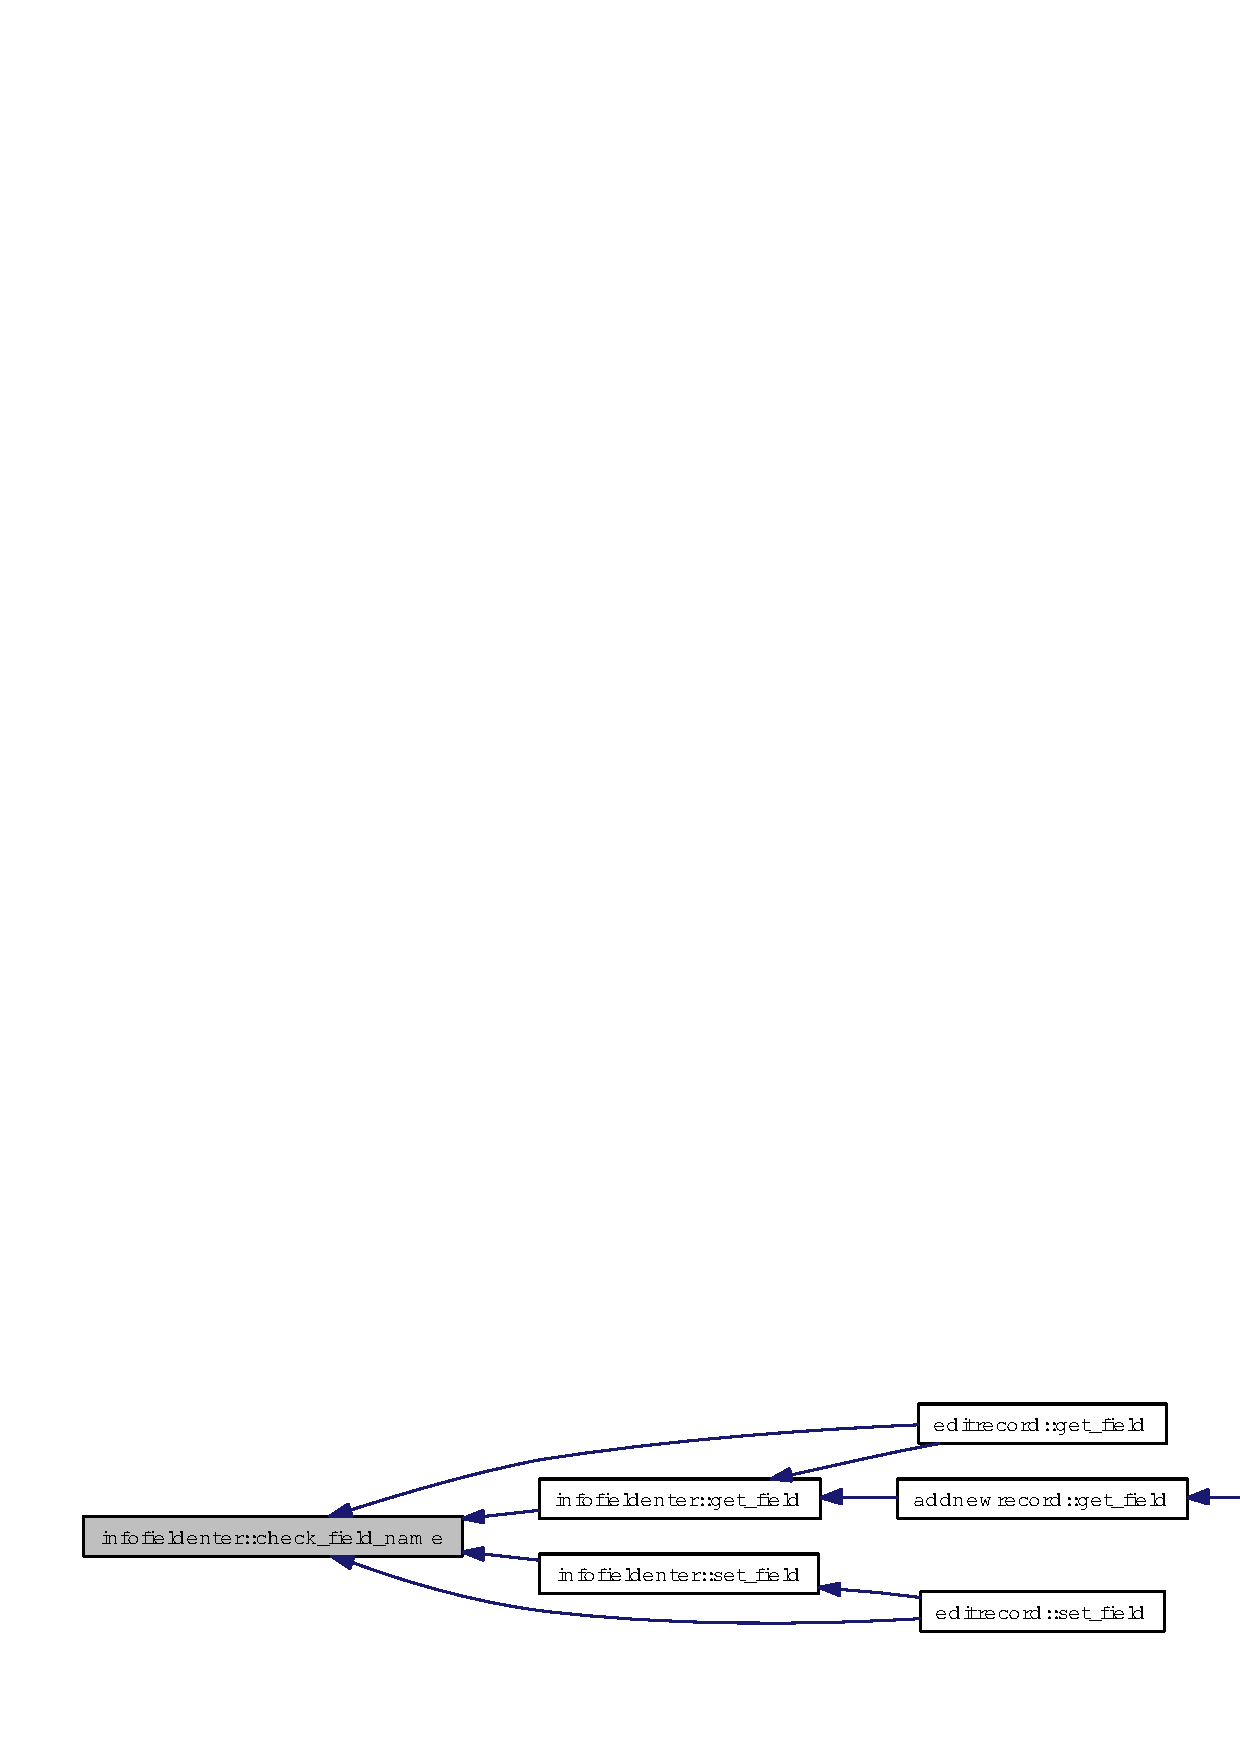
\includegraphics[width=404pt]{classinfofieldenter_1020b1777a4f93a10b5c04308625e62c_icgraph}
\end{center}
\end{figure}
\index{infofieldenter@{infofieldenter}!get_field@{get\_\-field}}
\index{get_field@{get\_\-field}!infofieldenter@{infofieldenter}}
\subsubsection{\setlength{\rightskip}{0pt plus 5cm}QString infofieldenter::get\_\-field (QString {\em name})}\label{classinfofieldenter_9ce895ba08dedfe227c839c56c2cb3b7}




Definition at line 170 of file infofieldenter.cpp.

References check\_\-field\_\-name(), critical\_\-error(), recordauthor, recordname, recordtags, and recordurl.

Referenced by editrecord::get\_\-field(), addnewrecord::get\_\-field(), editrecord::ok\_\-click(), and addnewrecord::ok\_\-click().

Here is the call graph for this function:\begin{figure}[H]
\begin{center}
\leavevmode
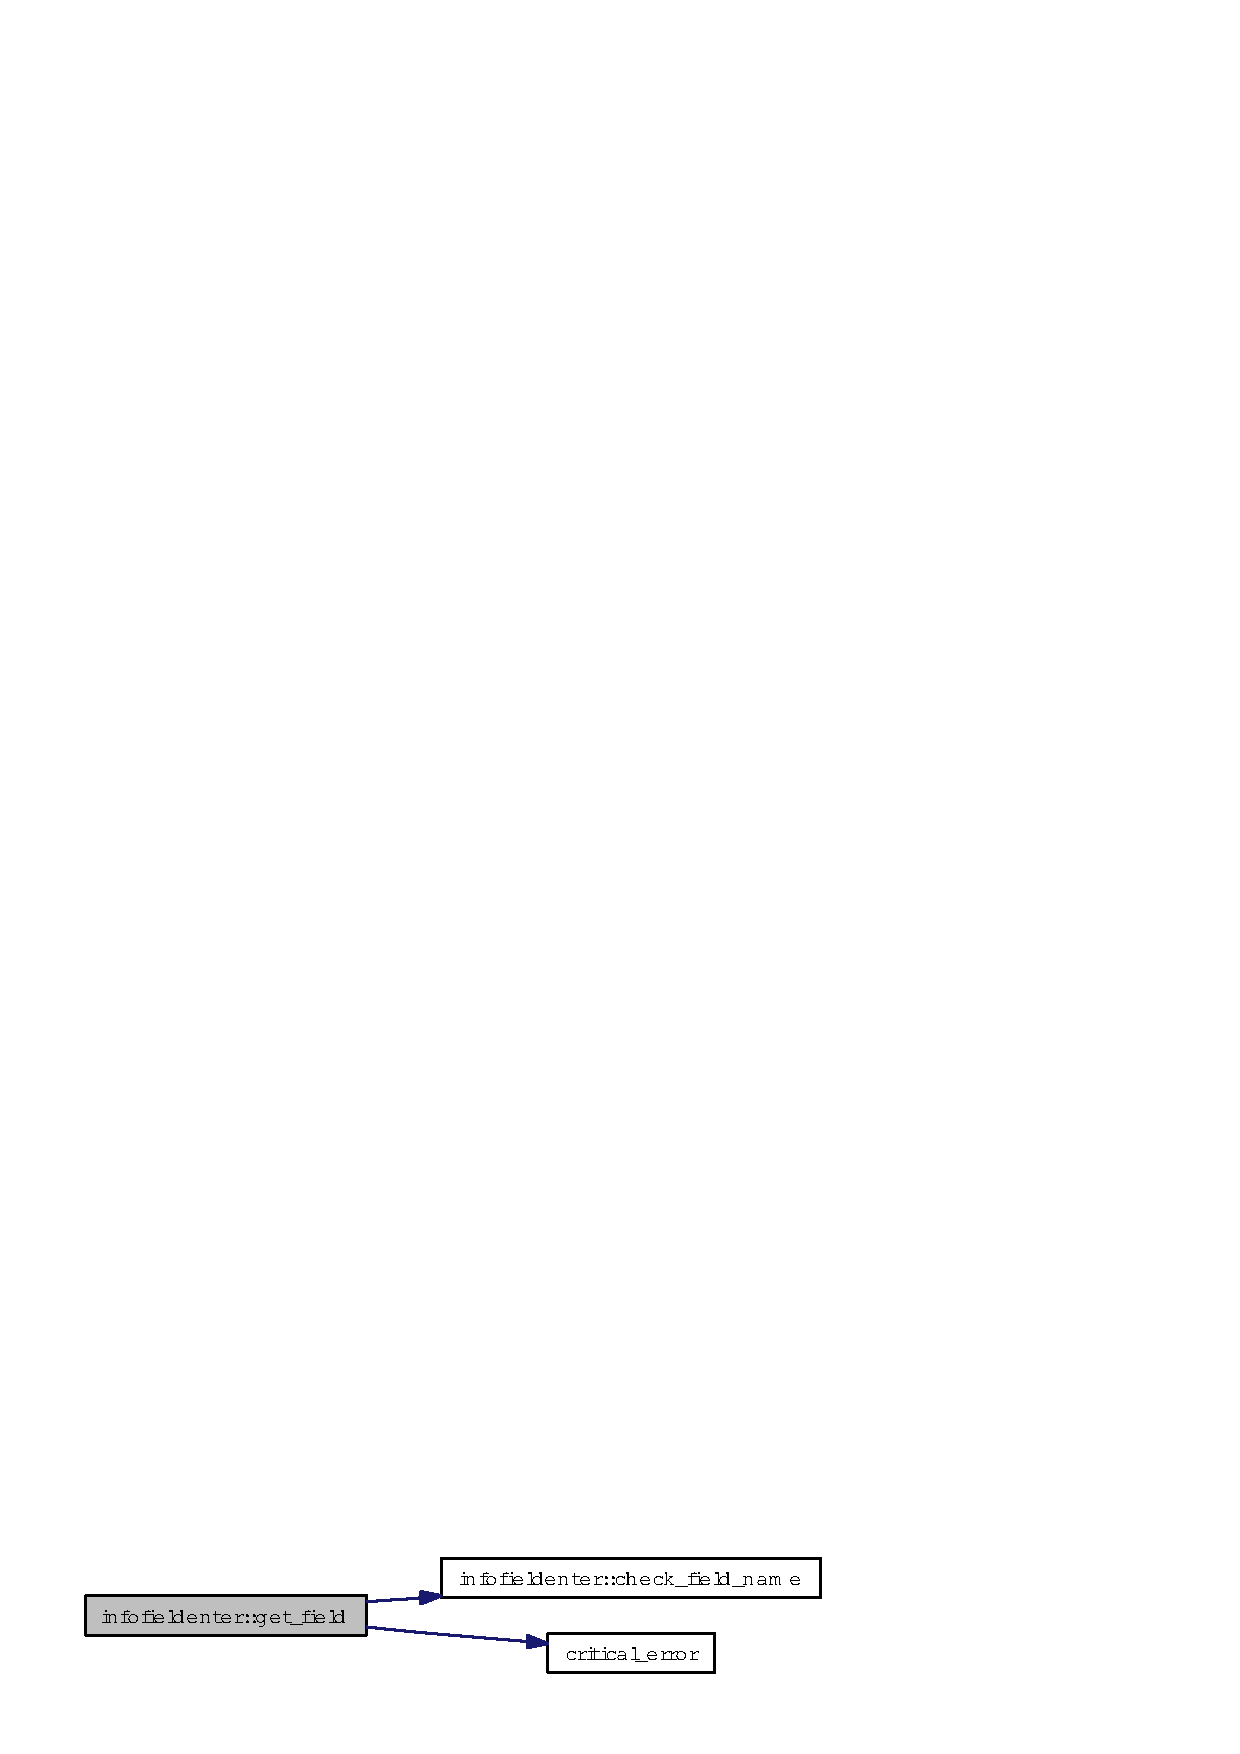
\includegraphics[width=199pt]{classinfofieldenter_9ce895ba08dedfe227c839c56c2cb3b7_cgraph}
\end{center}
\end{figure}


Here is the caller graph for this function:\begin{figure}[H]
\begin{center}
\leavevmode
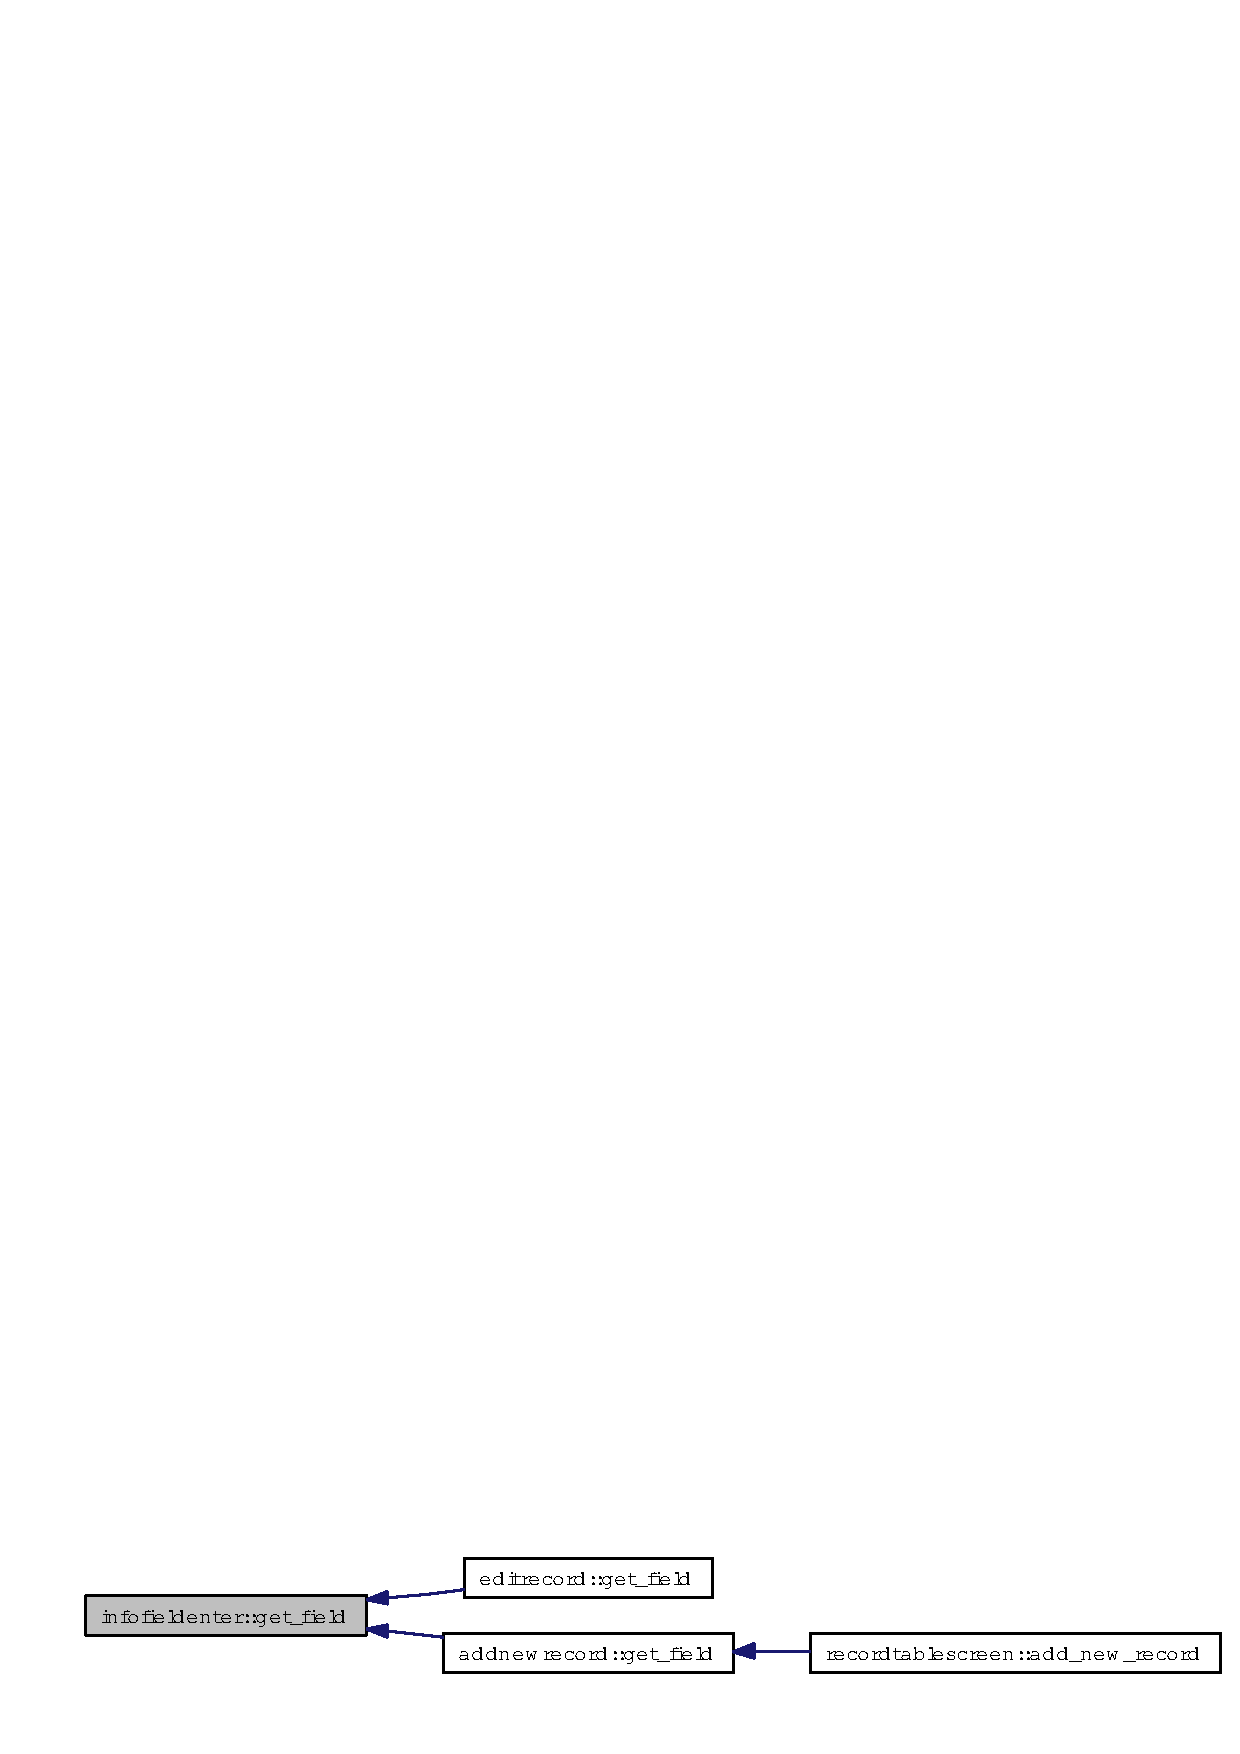
\includegraphics[width=295pt]{classinfofieldenter_9ce895ba08dedfe227c839c56c2cb3b7_icgraph}
\end{center}
\end{figure}
\index{infofieldenter@{infofieldenter}!set_field@{set\_\-field}}
\index{set_field@{set\_\-field}!infofieldenter@{infofieldenter}}
\subsubsection{\setlength{\rightskip}{0pt plus 5cm}void infofieldenter::set\_\-field (QString {\em name}, QString {\em value})}\label{classinfofieldenter_54f0af0d041c157e120c6d2521e25a8a}




Definition at line 186 of file infofieldenter.cpp.

References check\_\-field\_\-name(), critical\_\-error(), recordauthor, recordname, recordtags, and recordurl.

Referenced by editrecord::set\_\-field().

Here is the call graph for this function:\begin{figure}[H]
\begin{center}
\leavevmode
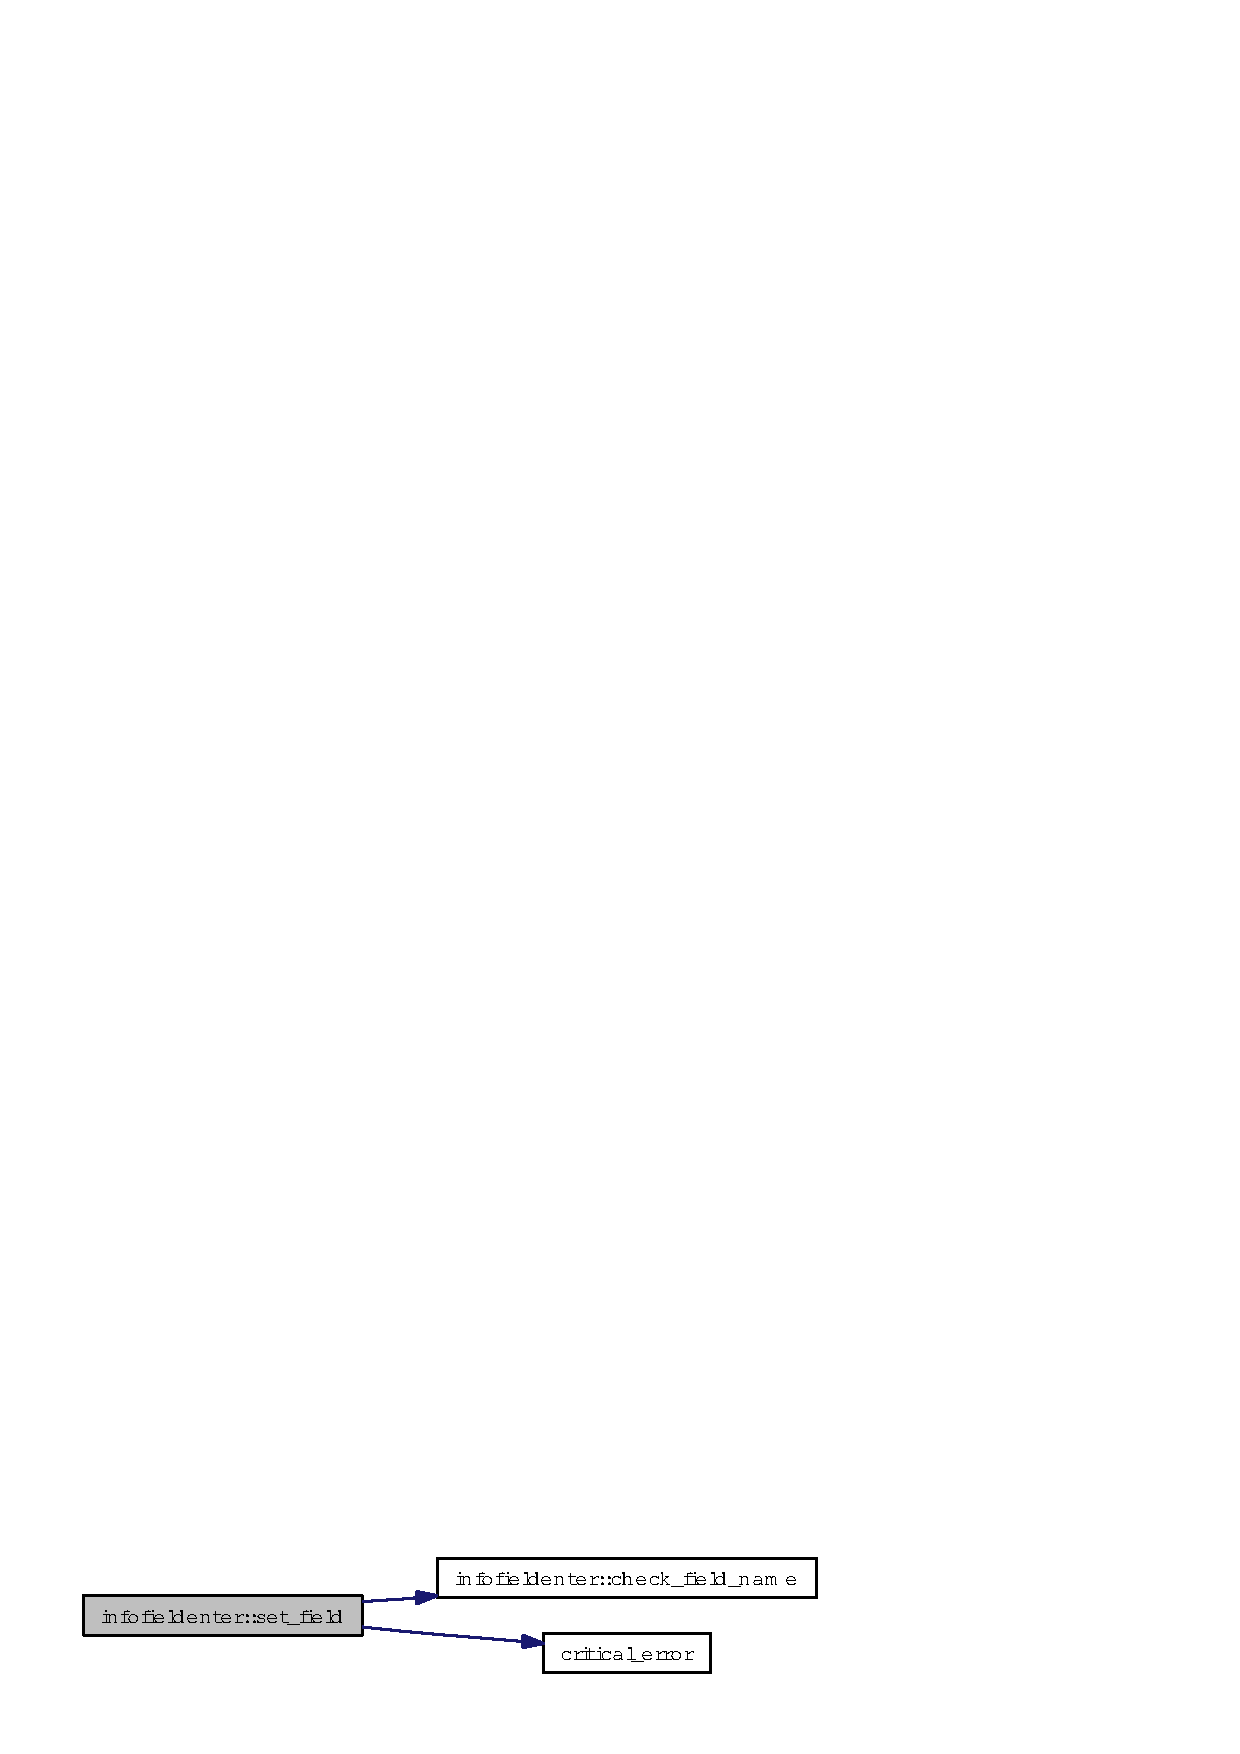
\includegraphics[width=198pt]{classinfofieldenter_54f0af0d041c157e120c6d2521e25a8a_cgraph}
\end{center}
\end{figure}


Here is the caller graph for this function:\begin{figure}[H]
\begin{center}
\leavevmode
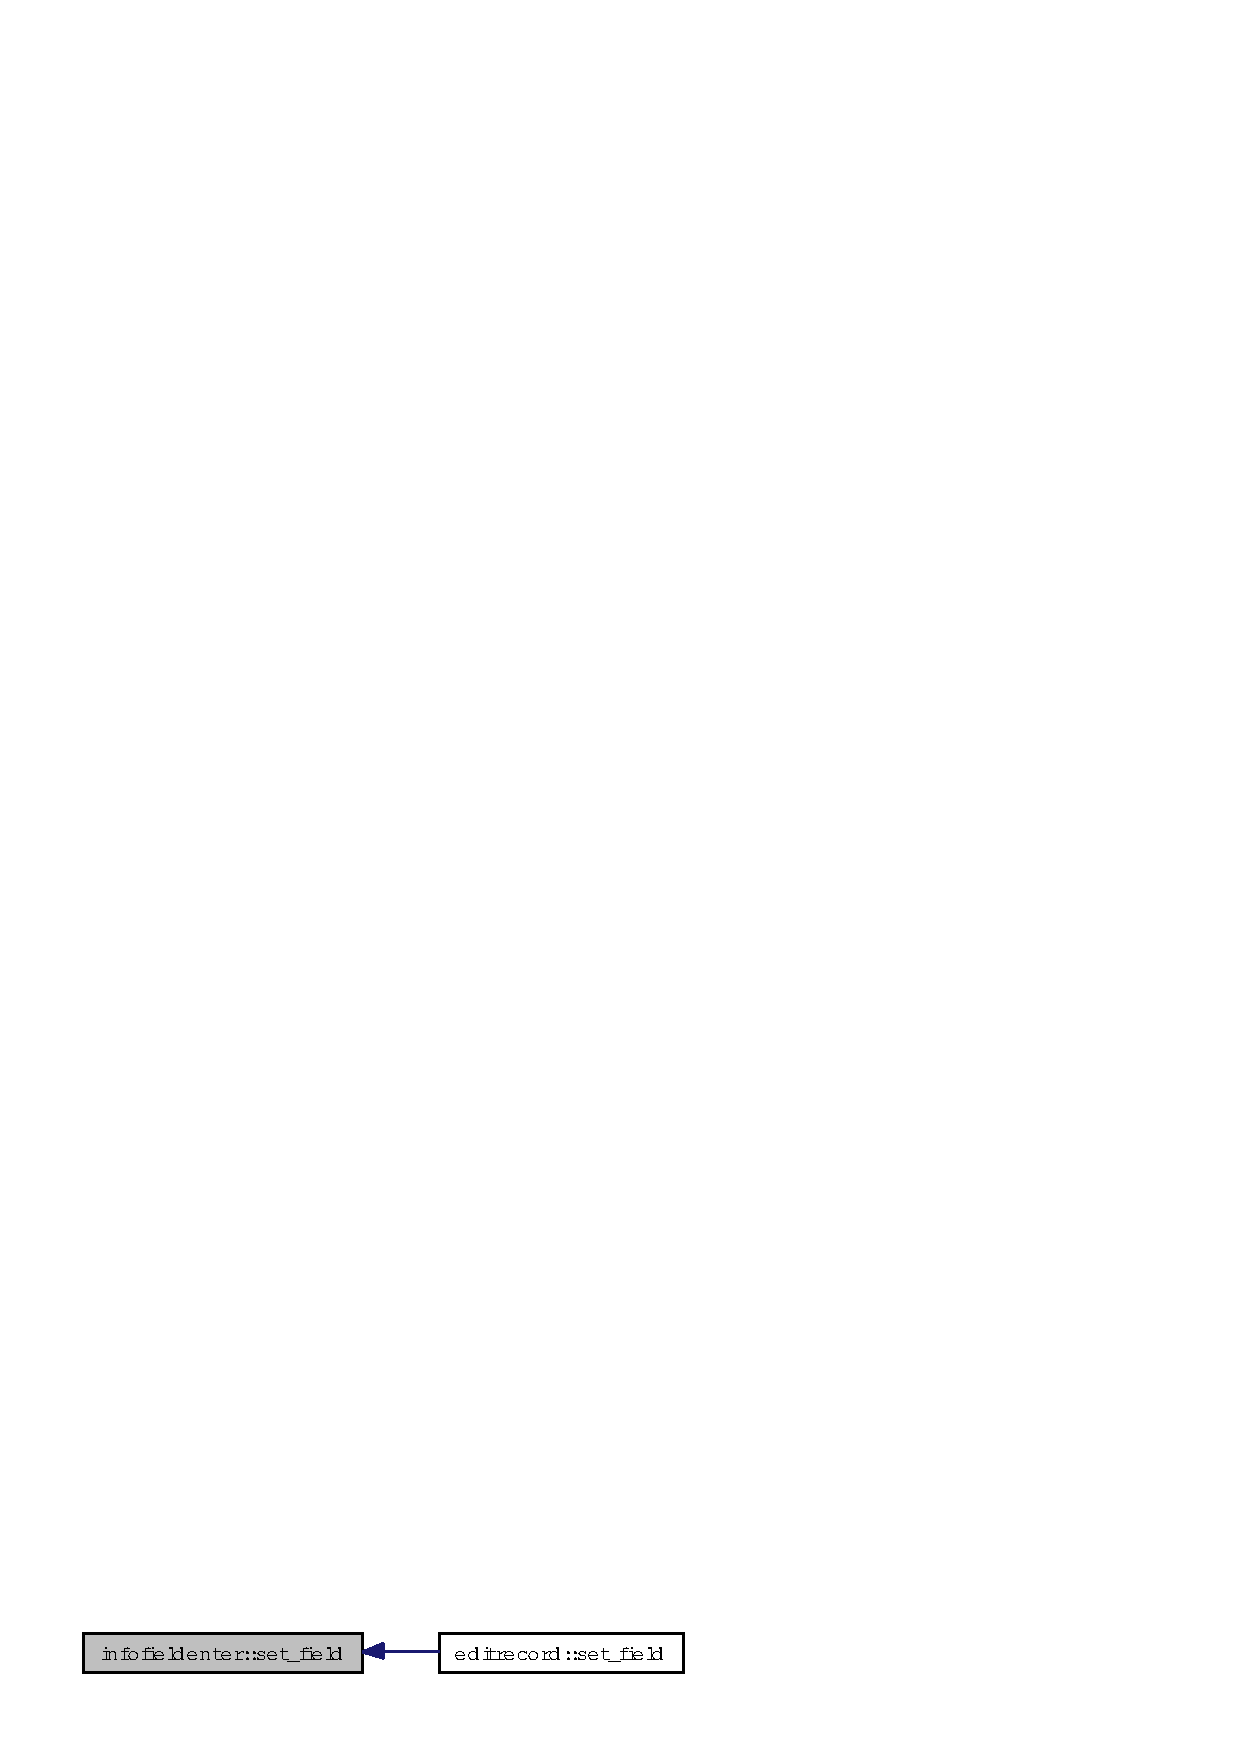
\includegraphics[width=166pt]{classinfofieldenter_54f0af0d041c157e120c6d2521e25a8a_icgraph}
\end{center}
\end{figure}
\index{infofieldenter@{infofieldenter}!expand_info_click@{expand\_\-info\_\-click}}
\index{expand_info_click@{expand\_\-info\_\-click}!infofieldenter@{infofieldenter}}
\subsubsection{\setlength{\rightskip}{0pt plus 5cm}void infofieldenter::expand\_\-info\_\-click (void)\hspace{0.3cm}{\tt  [slot]}}\label{classinfofieldenter_ce685991cc56e7c4bc7f0a3ef51d06a0}




Definition at line 129 of file infofieldenter.cpp.

References expand\_\-info, expand\_\-info\_\-on\_\-display(), appconfig::get\_\-addnewrecord\_\-expand\_\-info(), mytetraconfig, and appconfig::set\_\-addnewrecord\_\-expand\_\-info().

Referenced by setup\_\-signals().\index{infofieldenter@{infofieldenter}!setup_ui@{setup\_\-ui}}
\index{setup_ui@{setup\_\-ui}!infofieldenter@{infofieldenter}}
\subsubsection{\setlength{\rightskip}{0pt plus 5cm}void infofieldenter::setup\_\-ui (void)\hspace{0.3cm}{\tt  [private]}}\label{classinfofieldenter_108d06e5be71bc7208f6b867d0c487d2}




Definition at line 22 of file infofieldenter.cpp.

References expand\_\-info, appconfig::get\_\-addnewrecord\_\-expand\_\-info(), imin(), mytetraconfig, recordauthor, recordauthor\_\-label, recordname, recordname\_\-label, recordtags, recordtags\_\-label, recordurl, and recordurl\_\-label.

Referenced by infofieldenter().

Here is the call graph for this function:\begin{figure}[H]
\begin{center}
\leavevmode
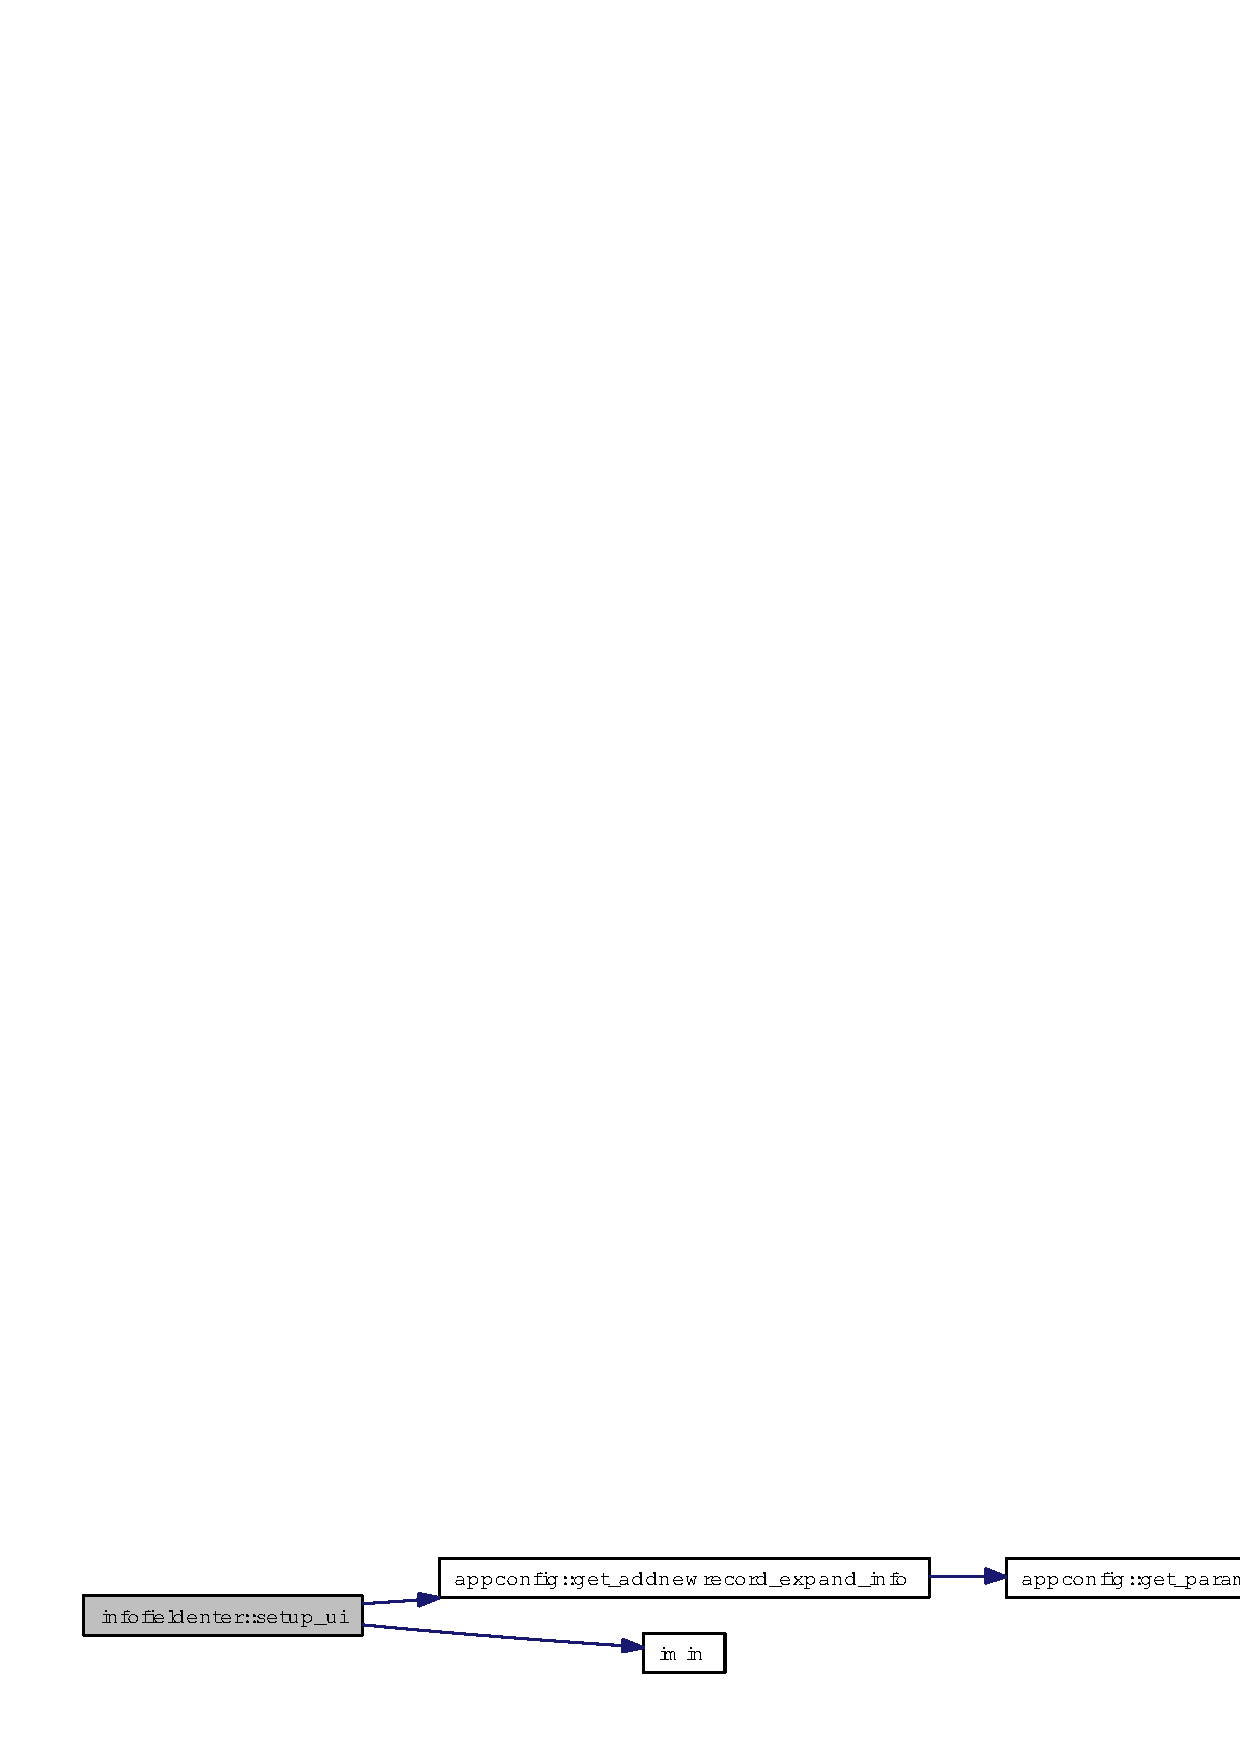
\includegraphics[width=376pt]{classinfofieldenter_108d06e5be71bc7208f6b867d0c487d2_cgraph}
\end{center}
\end{figure}


Here is the caller graph for this function:\begin{figure}[H]
\begin{center}
\leavevmode
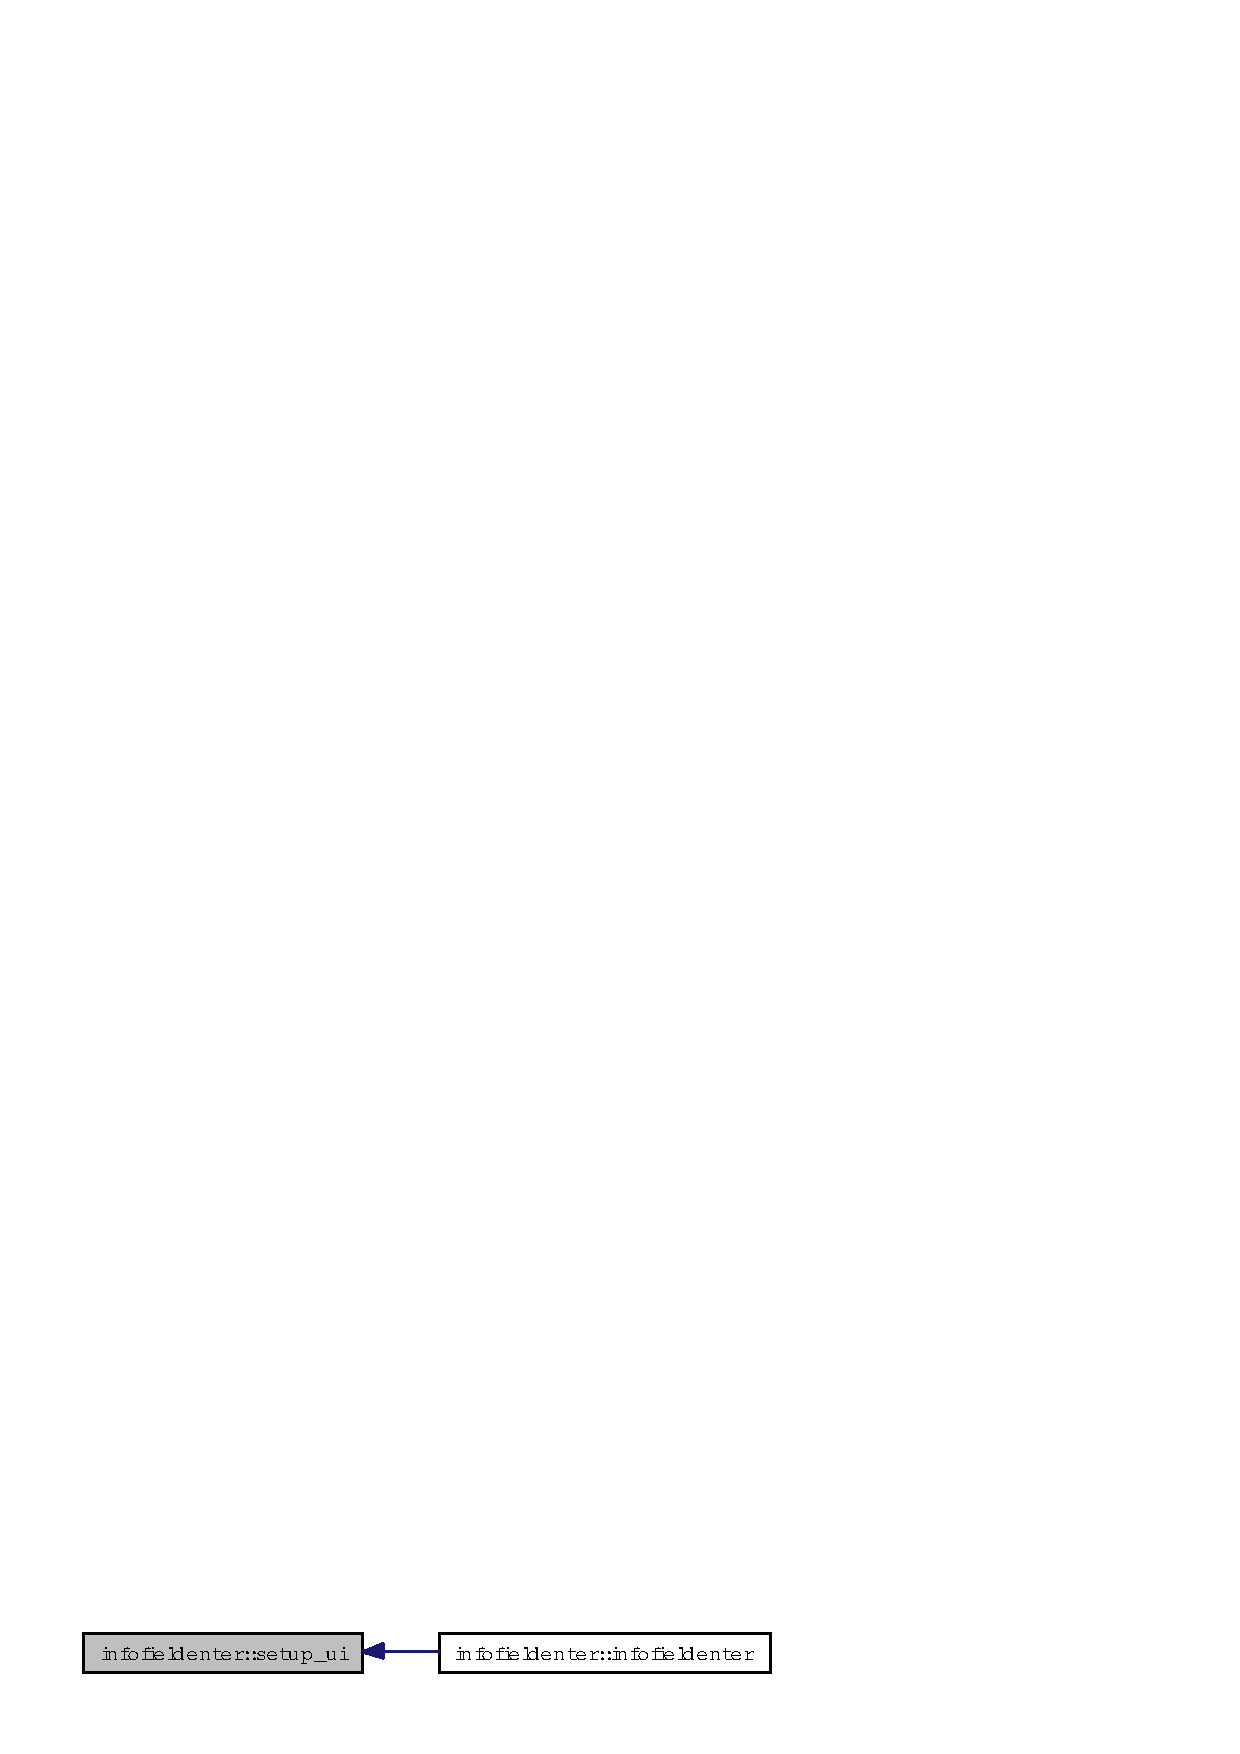
\includegraphics[width=187pt]{classinfofieldenter_108d06e5be71bc7208f6b867d0c487d2_icgraph}
\end{center}
\end{figure}
\index{infofieldenter@{infofieldenter}!setup_signals@{setup\_\-signals}}
\index{setup_signals@{setup\_\-signals}!infofieldenter@{infofieldenter}}
\subsubsection{\setlength{\rightskip}{0pt plus 5cm}void infofieldenter::setup\_\-signals (void)\hspace{0.3cm}{\tt  [private]}}\label{classinfofieldenter_6d4a65c882986cfaa951680c354e0ba7}




Definition at line 63 of file infofieldenter.cpp.

References expand\_\-info, and expand\_\-info\_\-click().

Referenced by infofieldenter().

Here is the caller graph for this function:\begin{figure}[H]
\begin{center}
\leavevmode
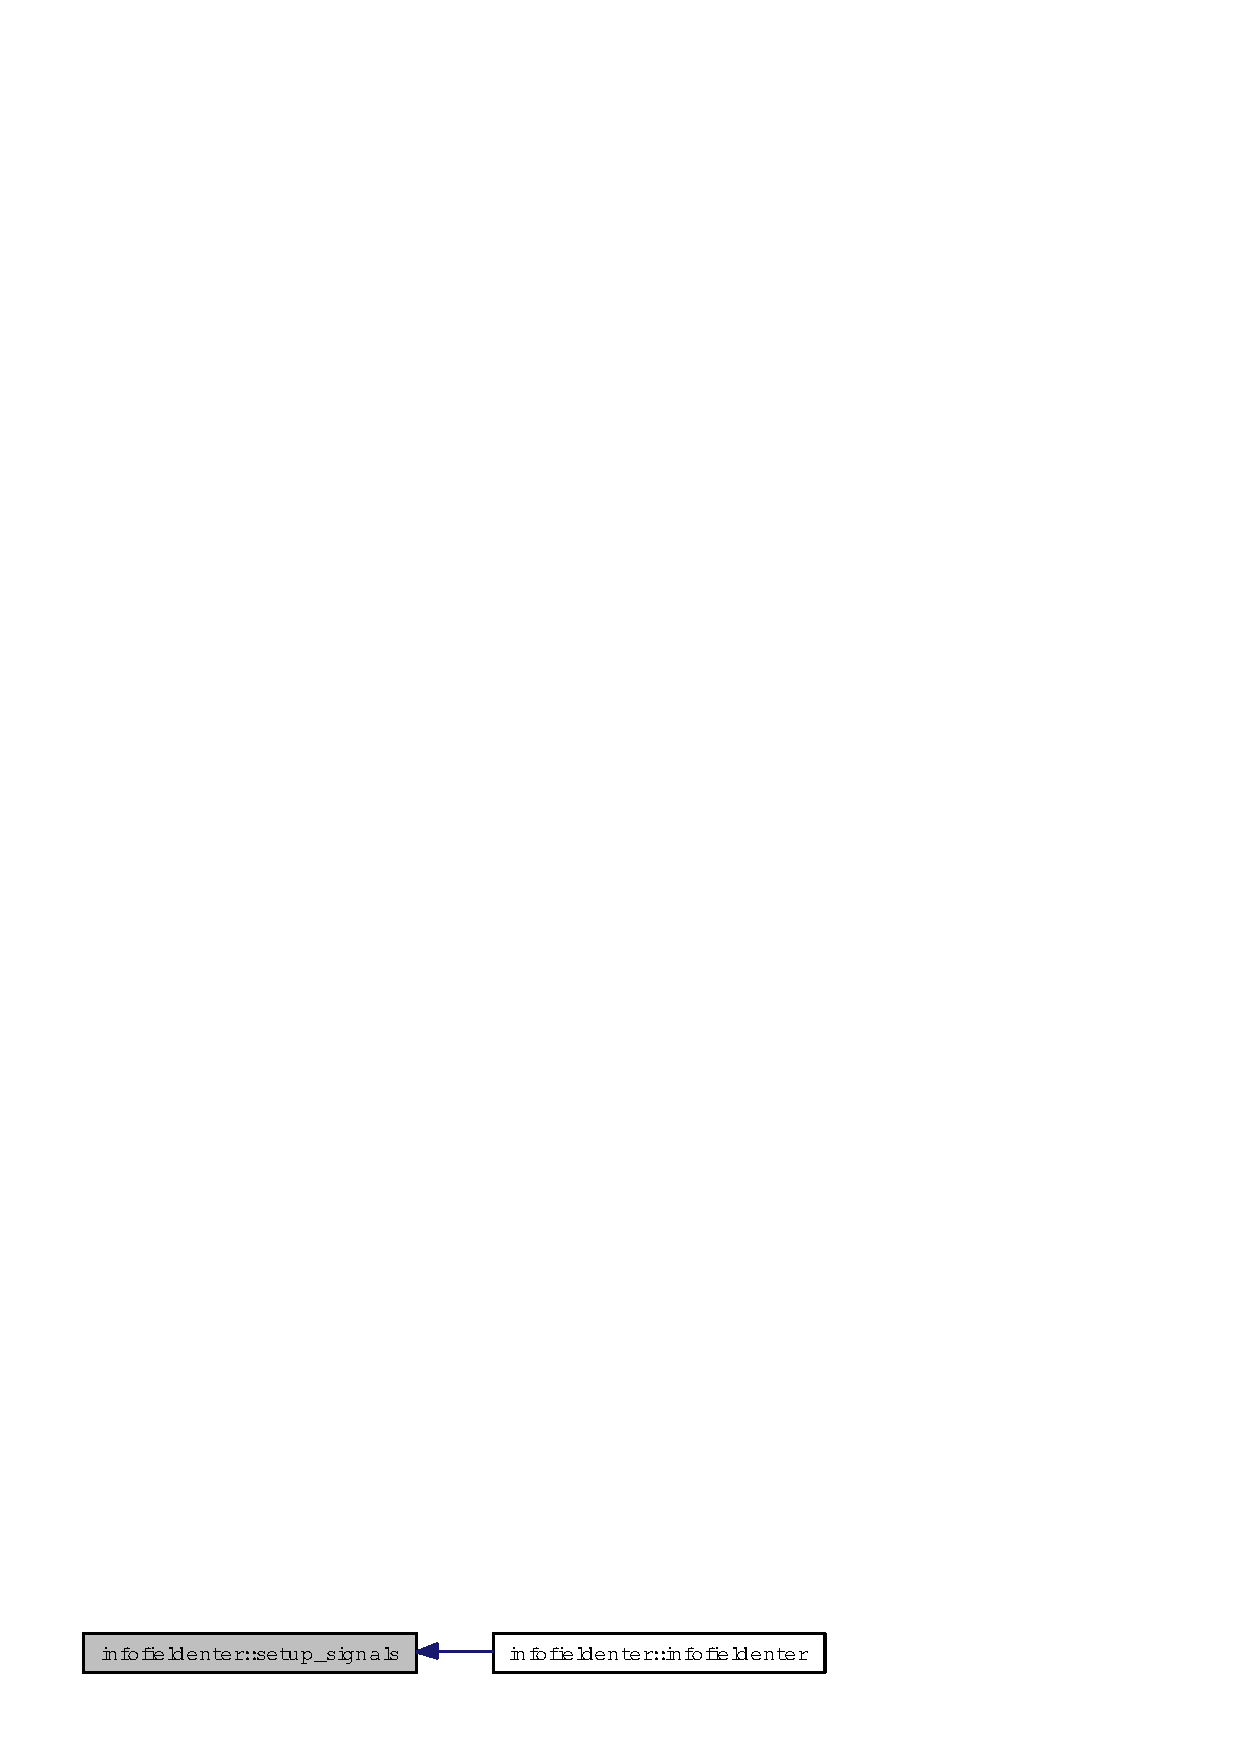
\includegraphics[width=200pt]{classinfofieldenter_6d4a65c882986cfaa951680c354e0ba7_icgraph}
\end{center}
\end{figure}
\index{infofieldenter@{infofieldenter}!assembly@{assembly}}
\index{assembly@{assembly}!infofieldenter@{infofieldenter}}
\subsubsection{\setlength{\rightskip}{0pt plus 5cm}void infofieldenter::assembly (void)\hspace{0.3cm}{\tt  [private]}}\label{classinfofieldenter_22f8772335566084852d85bcc0bf8963}




Definition at line 70 of file infofieldenter.cpp.

References expand\_\-info, expand\_\-info\_\-on\_\-display(), appconfig::get\_\-addnewrecord\_\-expand\_\-info(), infofieldlayout, mytetraconfig, recordauthor, recordauthor\_\-label, recordname, recordname\_\-label, recordtags, recordtags\_\-label, recordurl, and recordurl\_\-label.

Referenced by infofieldenter().

Here is the call graph for this function:\begin{figure}[H]
\begin{center}
\leavevmode
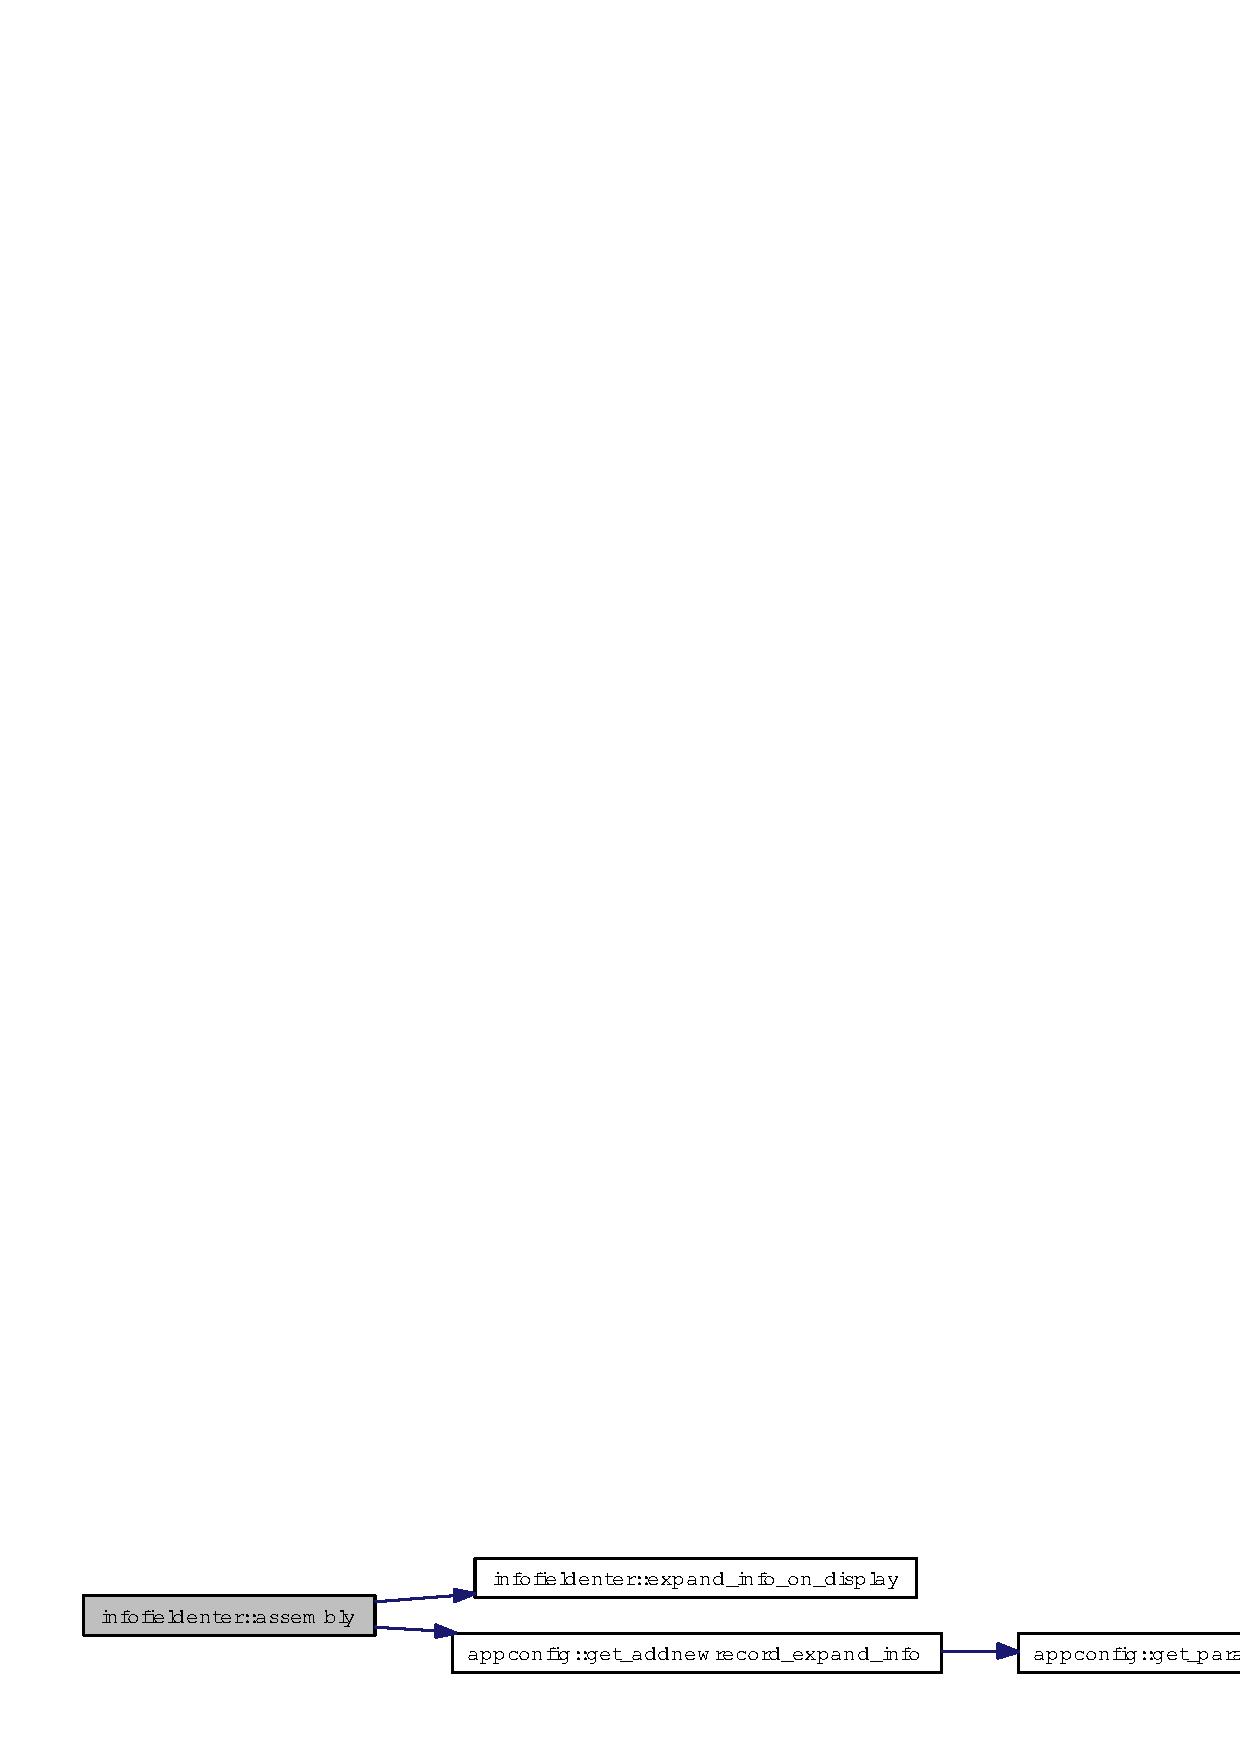
\includegraphics[width=379pt]{classinfofieldenter_22f8772335566084852d85bcc0bf8963_cgraph}
\end{center}
\end{figure}


Here is the caller graph for this function:\begin{figure}[H]
\begin{center}
\leavevmode
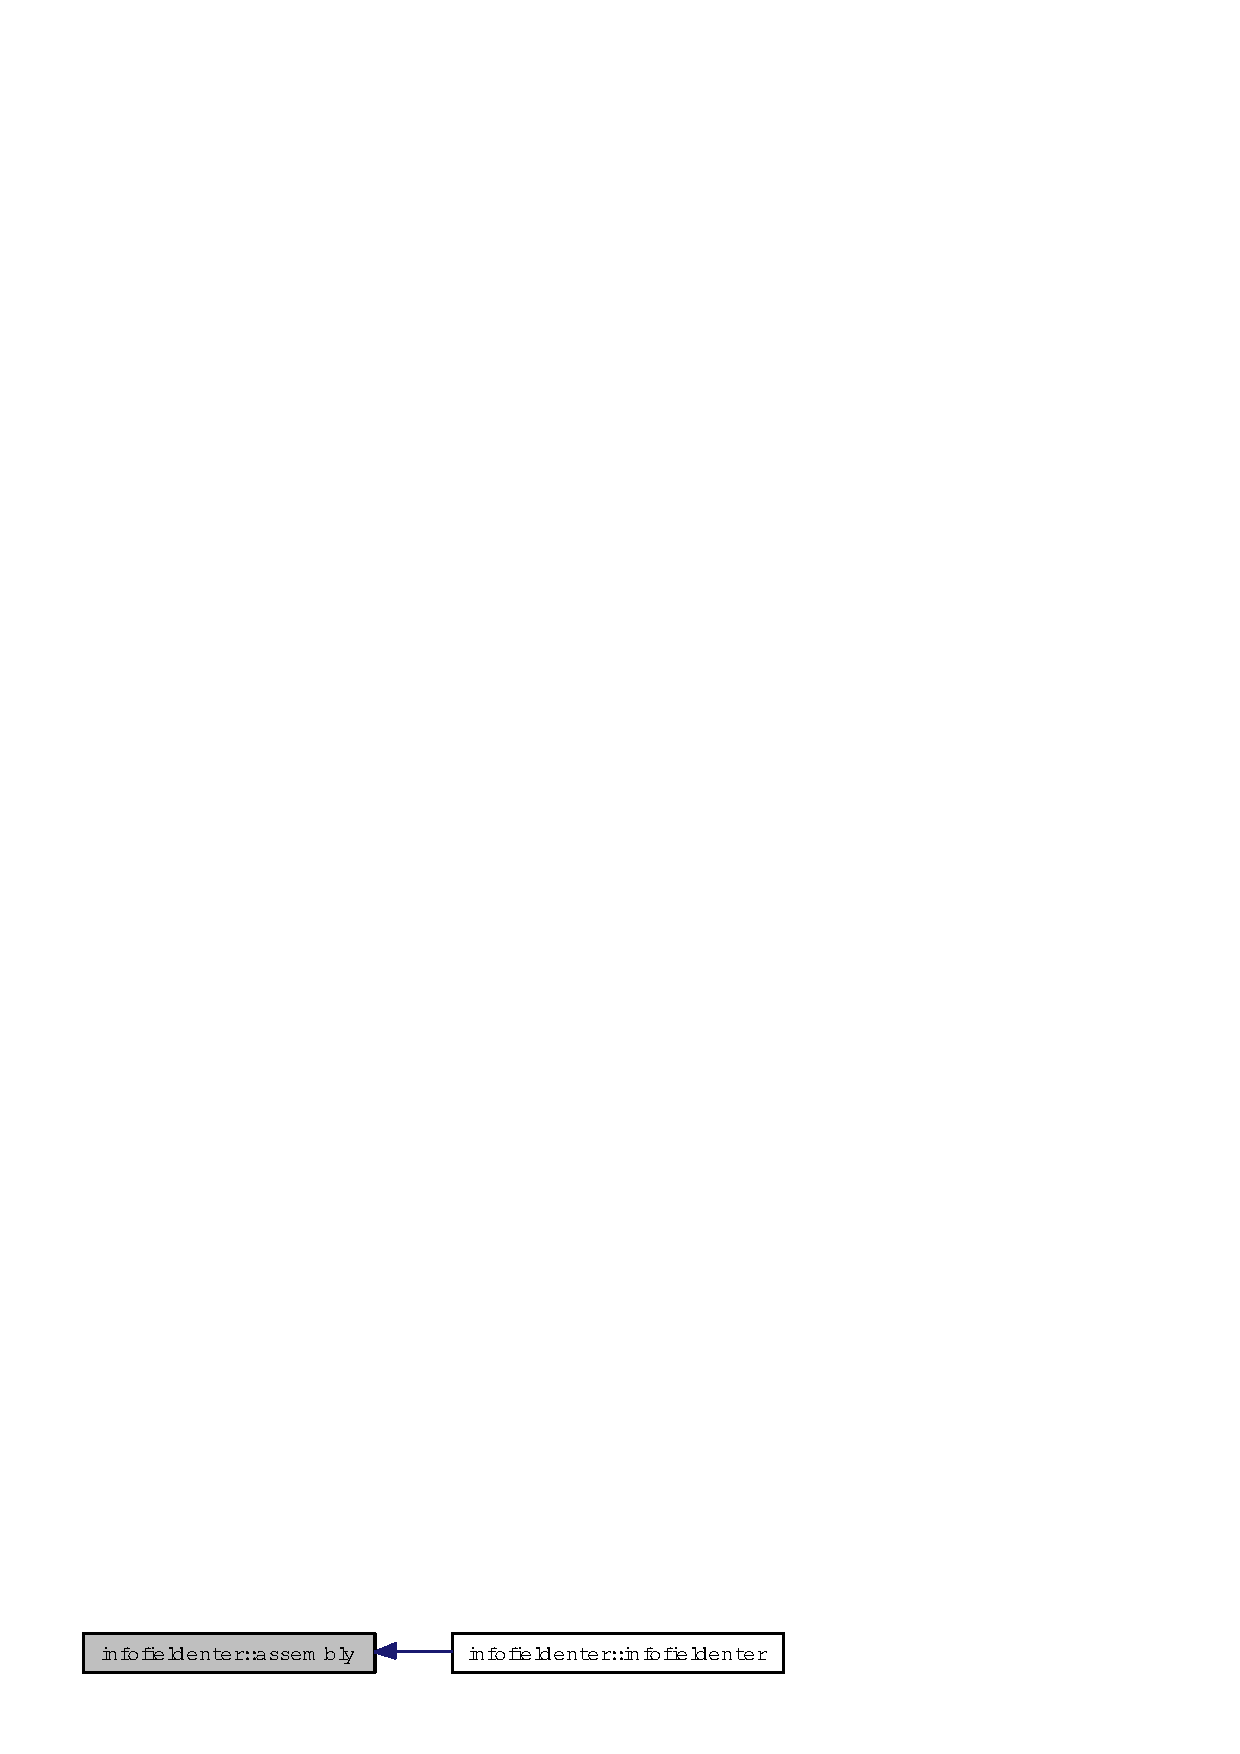
\includegraphics[width=190pt]{classinfofieldenter_22f8772335566084852d85bcc0bf8963_icgraph}
\end{center}
\end{figure}
\index{infofieldenter@{infofieldenter}!expand_info_on_display@{expand\_\-info\_\-on\_\-display}}
\index{expand_info_on_display@{expand\_\-info\_\-on\_\-display}!infofieldenter@{infofieldenter}}
\subsubsection{\setlength{\rightskip}{0pt plus 5cm}void infofieldenter::expand\_\-info\_\-on\_\-display (QString {\em expand})\hspace{0.3cm}{\tt  [private]}}\label{classinfofieldenter_1293795de93ff8d6810a658e80e15069}




Definition at line 109 of file infofieldenter.cpp.

References recordauthor, recordauthor\_\-label, recordtags, recordtags\_\-label, recordurl, and recordurl\_\-label.

Referenced by assembly(), and expand\_\-info\_\-click().

Here is the caller graph for this function:\begin{figure}[H]
\begin{center}
\leavevmode
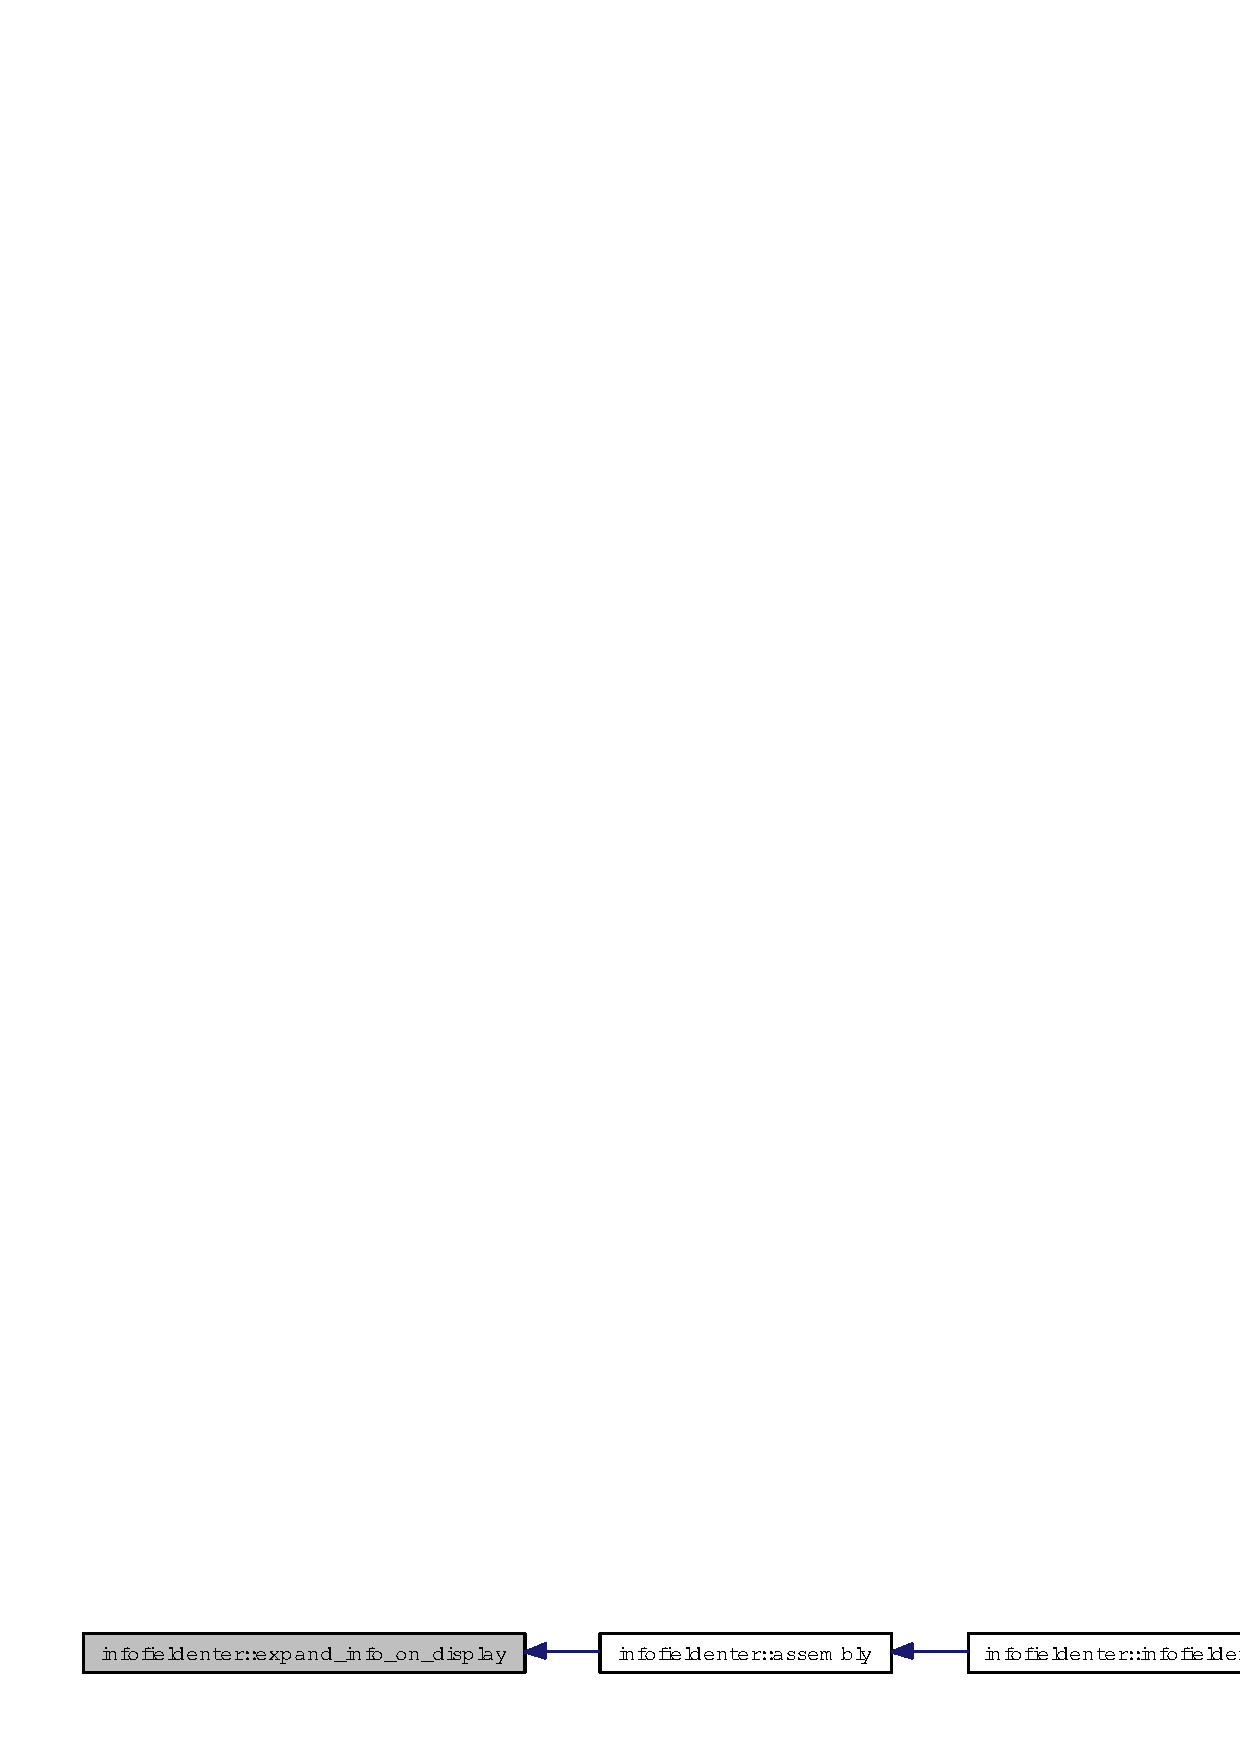
\includegraphics[width=314pt]{classinfofieldenter_1293795de93ff8d6810a658e80e15069_icgraph}
\end{center}
\end{figure}


\subsection{Member Data Documentation}
\index{infofieldenter@{infofieldenter}!recordname_label@{recordname\_\-label}}
\index{recordname_label@{recordname\_\-label}!infofieldenter@{infofieldenter}}
\subsubsection{\setlength{\rightskip}{0pt plus 5cm}QLabel$\ast$ {\bf infofieldenter::recordname\_\-label}\hspace{0.3cm}{\tt  [private]}}\label{classinfofieldenter_5d482d92e5efc647a4e022ade9899ead}




Definition at line 36 of file infofieldenter.h.

Referenced by assembly(), and setup\_\-ui().\index{infofieldenter@{infofieldenter}!recordname@{recordname}}
\index{recordname@{recordname}!infofieldenter@{infofieldenter}}
\subsubsection{\setlength{\rightskip}{0pt plus 5cm}QLine\-Edit$\ast$ {\bf infofieldenter::recordname}\hspace{0.3cm}{\tt  [private]}}\label{classinfofieldenter_7af2f90d29958f18b4f31281e3f11e3c}




Definition at line 37 of file infofieldenter.h.

Referenced by assembly(), get\_\-field(), set\_\-field(), set\_\-focus\_\-to\_\-start(), and setup\_\-ui().\index{infofieldenter@{infofieldenter}!recordauthor_label@{recordauthor\_\-label}}
\index{recordauthor_label@{recordauthor\_\-label}!infofieldenter@{infofieldenter}}
\subsubsection{\setlength{\rightskip}{0pt plus 5cm}QLabel$\ast$ {\bf infofieldenter::recordauthor\_\-label}\hspace{0.3cm}{\tt  [private]}}\label{classinfofieldenter_88635e70eb97d755fe51097aab986404}




Definition at line 40 of file infofieldenter.h.

Referenced by assembly(), expand\_\-info\_\-on\_\-display(), and setup\_\-ui().\index{infofieldenter@{infofieldenter}!recordauthor@{recordauthor}}
\index{recordauthor@{recordauthor}!infofieldenter@{infofieldenter}}
\subsubsection{\setlength{\rightskip}{0pt plus 5cm}QLine\-Edit$\ast$ {\bf infofieldenter::recordauthor}\hspace{0.3cm}{\tt  [private]}}\label{classinfofieldenter_bbb59d8a51ad8f9392e59644a6222032}




Definition at line 41 of file infofieldenter.h.

Referenced by assembly(), expand\_\-info\_\-on\_\-display(), get\_\-field(), set\_\-field(), and setup\_\-ui().\index{infofieldenter@{infofieldenter}!recordurl_label@{recordurl\_\-label}}
\index{recordurl_label@{recordurl\_\-label}!infofieldenter@{infofieldenter}}
\subsubsection{\setlength{\rightskip}{0pt plus 5cm}QLabel$\ast$ {\bf infofieldenter::recordurl\_\-label}\hspace{0.3cm}{\tt  [private]}}\label{classinfofieldenter_f886fba61763496c28db9d272d50221f}




Definition at line 44 of file infofieldenter.h.

Referenced by assembly(), expand\_\-info\_\-on\_\-display(), and setup\_\-ui().\index{infofieldenter@{infofieldenter}!recordurl@{recordurl}}
\index{recordurl@{recordurl}!infofieldenter@{infofieldenter}}
\subsubsection{\setlength{\rightskip}{0pt plus 5cm}QLine\-Edit$\ast$ {\bf infofieldenter::recordurl}\hspace{0.3cm}{\tt  [private]}}\label{classinfofieldenter_faa3049ed6ee380bde57cd54e4673052}




Definition at line 45 of file infofieldenter.h.

Referenced by assembly(), expand\_\-info\_\-on\_\-display(), get\_\-field(), set\_\-field(), and setup\_\-ui().\index{infofieldenter@{infofieldenter}!recordtags_label@{recordtags\_\-label}}
\index{recordtags_label@{recordtags\_\-label}!infofieldenter@{infofieldenter}}
\subsubsection{\setlength{\rightskip}{0pt plus 5cm}QLabel$\ast$ {\bf infofieldenter::recordtags\_\-label}\hspace{0.3cm}{\tt  [private]}}\label{classinfofieldenter_aee4df3556027801ad97d16ebc51cfc8}




Definition at line 48 of file infofieldenter.h.

Referenced by assembly(), expand\_\-info\_\-on\_\-display(), and setup\_\-ui().\index{infofieldenter@{infofieldenter}!recordtags@{recordtags}}
\index{recordtags@{recordtags}!infofieldenter@{infofieldenter}}
\subsubsection{\setlength{\rightskip}{0pt plus 5cm}QLine\-Edit$\ast$ {\bf infofieldenter::recordtags}\hspace{0.3cm}{\tt  [private]}}\label{classinfofieldenter_8d04fa9810cddeab8154069924f51f52}




Definition at line 49 of file infofieldenter.h.

Referenced by assembly(), expand\_\-info\_\-on\_\-display(), get\_\-field(), set\_\-field(), and setup\_\-ui().\index{infofieldenter@{infofieldenter}!expand_info@{expand\_\-info}}
\index{expand_info@{expand\_\-info}!infofieldenter@{infofieldenter}}
\subsubsection{\setlength{\rightskip}{0pt plus 5cm}QTool\-Button$\ast$ {\bf infofieldenter::expand\_\-info}\hspace{0.3cm}{\tt  [private]}}\label{classinfofieldenter_d8caf1d9f6c55fda34df8ace07e48251}




Definition at line 52 of file infofieldenter.h.

Referenced by assembly(), expand\_\-info\_\-click(), setup\_\-signals(), and setup\_\-ui().\index{infofieldenter@{infofieldenter}!infofieldlayout@{infofieldlayout}}
\index{infofieldlayout@{infofieldlayout}!infofieldenter@{infofieldenter}}
\subsubsection{\setlength{\rightskip}{0pt plus 5cm}QGrid\-Layout$\ast$ {\bf infofieldenter::infofieldlayout}\hspace{0.3cm}{\tt  [private]}}\label{classinfofieldenter_430f081ceaa69eb3431a5abd2a11205e}




Definition at line 55 of file infofieldenter.h.

Referenced by assembly().

The documentation for this class was generated from the following files:\begin{CompactItemize}
\item 
{\bf infofieldenter.h}\item 
{\bf infofieldenter.cpp}\end{CompactItemize}
